\section{Alvin, Sandeep and a camera in U-bend}

\margininbox{U-bend 571}{
     \begin{itemize}
    \item Alvin Chow
    \item Sandeep Mavadia
    \end{itemize}}{\explo}

\passage{U-Bend 571} was first discovered and explored in 2000\sidenote{see The Hollow Mountain, page 120}. The remaining lead - a sharp, strongly draughting rift - was pushed in 2005\sidenote{detailed in the 2005 chapter of The Hollow Mountain}. It refused to yield to varying methods of persuasion that year - in Sandeep's own words they had to leave "the conquest of this cave for yet another day". 2007 would provide that day, when the cave was connected to \passage{Drugi Vhod} in \passage{Primadona}.


\begin{pagefigure}
      \checkoddpage \ifoddpage \forcerectofloat \else \forceversofloat \fi
    \centering
    \begin{subfigure}{0.49\textwidth}
        \frame{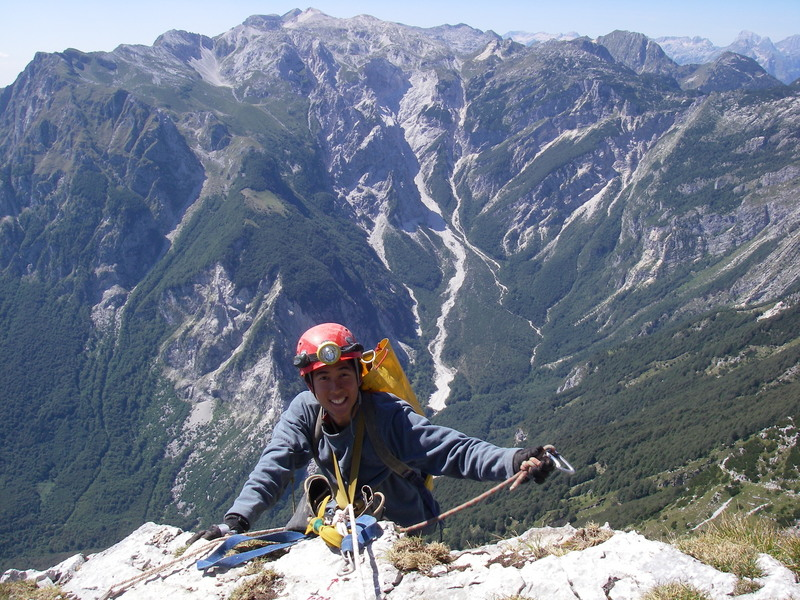
\includegraphics[width=\linewidth]{2007/ubend/sandeep mavadia - u-bend - IMGP0193--orig.jpg}}
        \caption{Alvin at the top of the cliff abseil.}
    \end{subfigure}
\hfill
    \begin{subfigure}{0.49\textwidth}
    \centering
        \frame{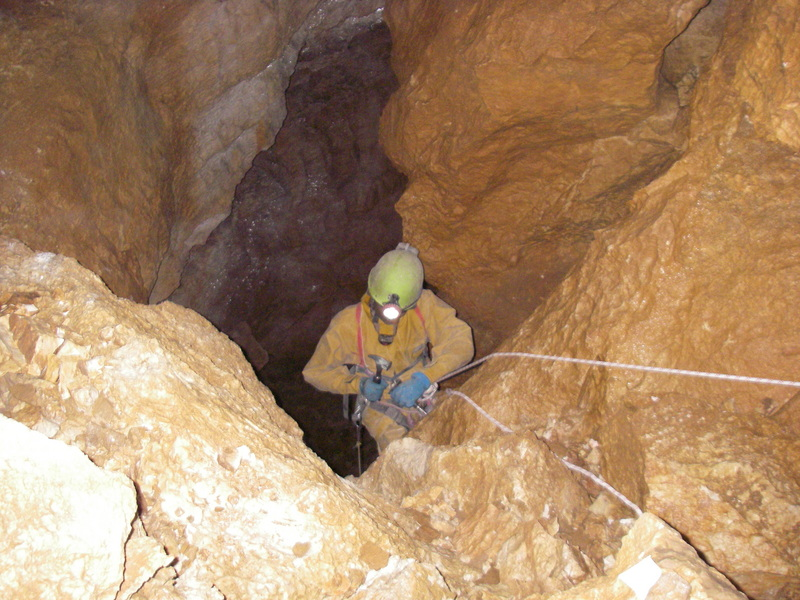
\includegraphics[width=\linewidth]{2007/ubend/sandeep mavadia - u-bend - IMGP0197--orig.jpg}}
        \caption{Sandeep placing a bolt.}
\end{subfigure}
\vfill
\begin{subfigure}{0.49\textwidth}
    \centering
        \frame{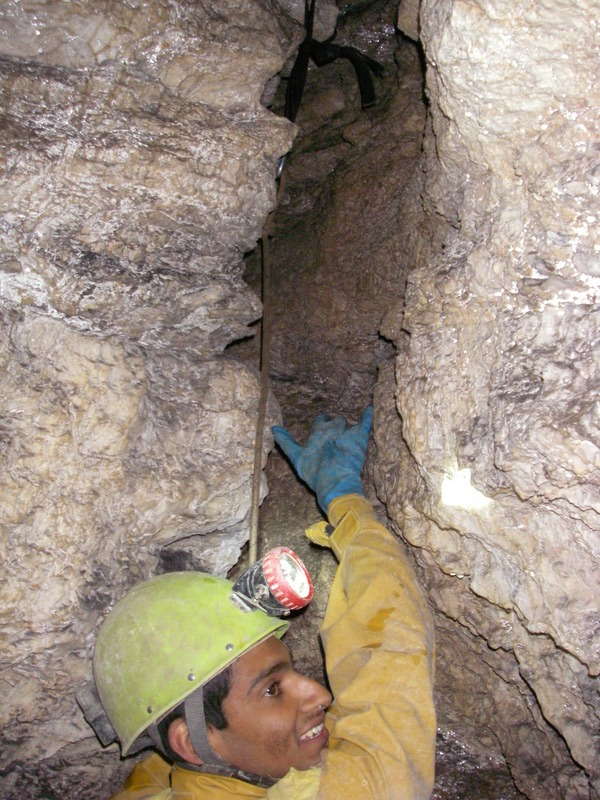
\includegraphics[width=\linewidth]{2007/ubend/sandeep mavadia - u-bend - IMGP0199--orig.jpg}}
        \caption{Sandeep highlights the size of the rift.}
\end{subfigure}
\hfill
\begin{subfigure}{0.49\textwidth}
    \centering
        \frame{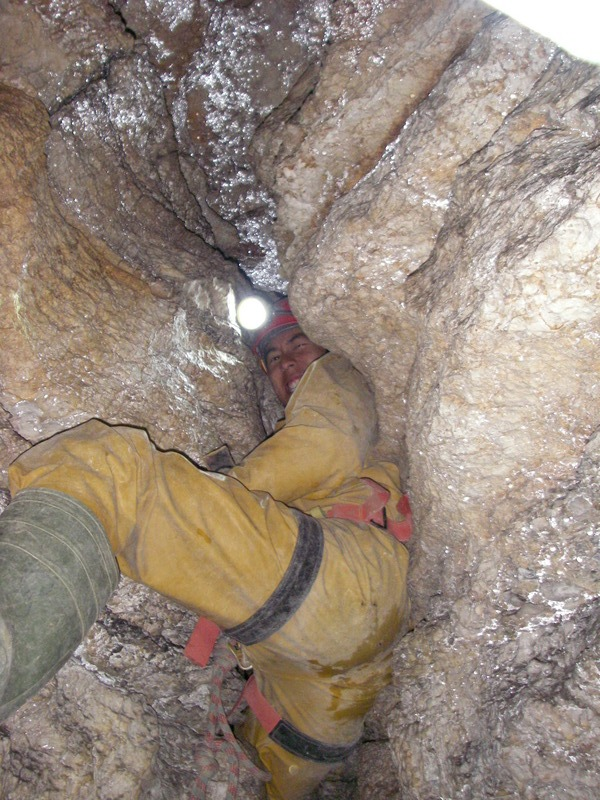
\includegraphics[width=\linewidth]{2007/ubend/sandeep mavadia - u-bend - IMGP0200--orig.jpg}}
        \caption{Alvin in a tight spot.}
    \end{subfigure}
\vfill
\caption{Pushing in \protect\passage{U-Bend}. \pic{Sandeep Mavadia / Alvin Chow}}
\end{pagefigure}


